 %RELATÓRIO DO PROJETO DE PROGRAMAÇAO ORIENTADA AOS OBJETOS 2019 - Carro UM Já!

%----------------------------------------------------------------------------------------------------------------------

\documentclass[a4paper,11pt]{report}
\usepackage[utf8]{inputenc}
\usepackage[portuguese]{babel}
\usepackage{graphicx}
\usepackage{hyperref}
\usepackage{float}
\usepackage{listings}


%----------------------------------------------------------------------------------------------------------------------

\usepackage{geometry}
 \geometry{
     a4paper,
     total={170mm,257mm},
     left=25mm,
     right=25mm,
     top=20mm,
 }

\graphicspath{{./base_images/}}

%----------------------------------------------------------------------------------------------------------------------

\begin{document}

%----------------------------------------------------------------------------------------------------------------------


\begin{titlepage}
    \center
    {

    \begin{figure}[t]
        \centering
        
\includegraphics[scale=0.4]{uminho.png}
        \label{img:logo}
        \vspace{2.0cm}
    \end{figure}

    \vspace{3.0cm}
    \textsc{\huge Programação Orientada Aos Objetos}\\[0.5cm]
    \textsc{\Large{Mestrado Integrado em Engenharia Informática}}\\[0.5cm]
    \vspace{2.0cm}
    \textsc{\Huge{UM carro Já!}}\\[0.5cm]
    
    \vspace{2.9cm}
    
    \textsc{\huge Grupo 25}\\[0.5cm]
        
    \vspace{0.5cm}
    
    \begin{figure}[htp]

        \centering
        
\includegraphics[width=.25\textwidth]{zizu.jpg}\hfill
        
\includegraphics[width=.25\textwidth]{paulob2.jpg}\hfill
        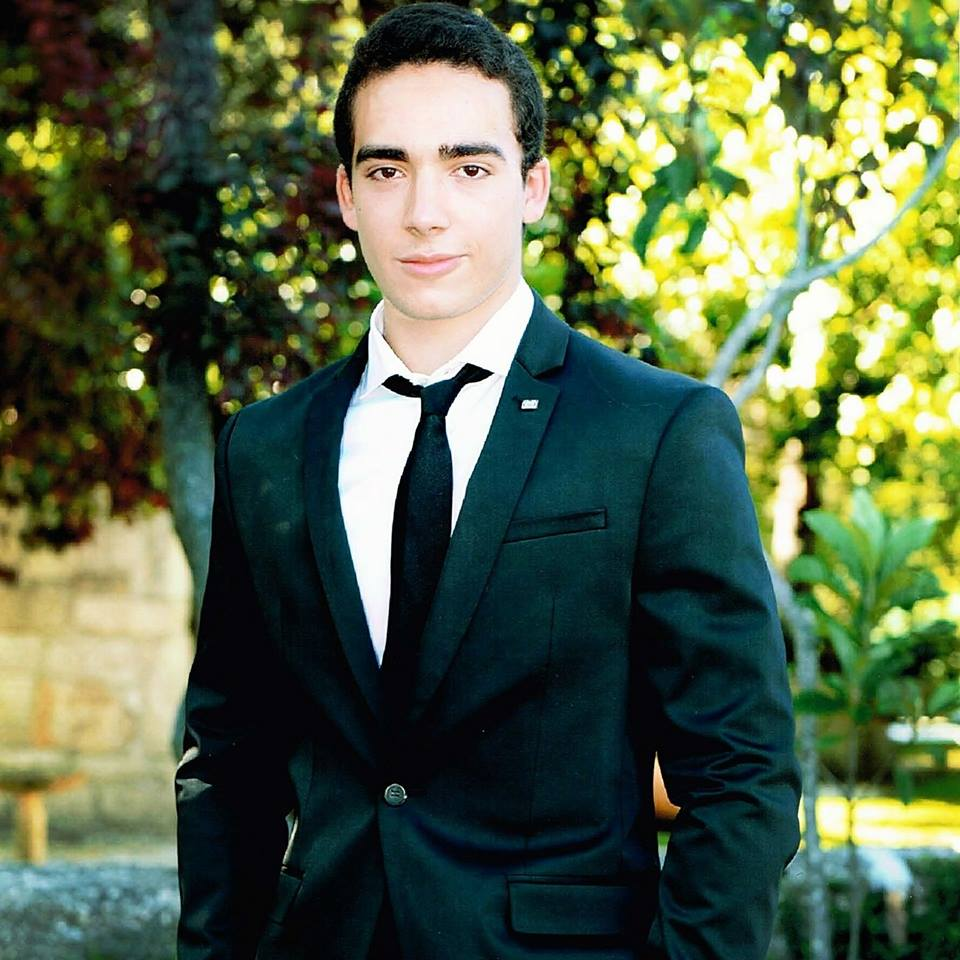
\includegraphics[width=.25\textwidth]{machado.jpg}

        \label{fig:figure3}

    \end{figure}
    
     \begin{flushleft}
        
         \textsc{\normalsize A85227 João Azevedo \hspace{1cm} A85729 Paulo Araújo \hspace{1cm} A83719 Pedro Machado}
    \end{flushleft}
    
        \vspace{1cm}
    \begin{flushright}
        Braga

        Maio 2019
    \end{flushright}

\date{\today}
}
\end{titlepage}

%----------------------------------------------------------------------------------------------------------------------

%Indice

\tableofcontents
\clearpage

%---------------------------------------------------------------------------------------------------------------------
%---------------------------------------------------------------------------------------------------------------------

% Introdução

\chapter{Introdução}

\hspace{0.50cm} Este trabalho foi realizado no âmbito da unidade curricular de Programação Orientada aos Objetos do curso de Mestrado Integrado em Engenharia Informática (MIEI). \par

\vspace{0.5cm}

Esta UC, assim como este trabalho prático, tinha como principal objetivo a utilização de conhecimentos Teóricos e 
Práticos relativos à programação por objetos na linguagem de programação java. 

\vspace{0.5cm}

Deste modo, foram importantes conhecimentos relativos à noção de objetos em POO, encapsulamento, classes e hierarquias de classes, herança e classes abstratas, herança simples, herança múltipla e interfaces. \par

\section{Objectivos}

\hspace{0.50cm} Neste trabalho pretende-se construir um serviço de aluguer de veículos particulares pela internet.  Na aplicação a desenvolver, um proprietário de um automóvel poderá registar o seu veiculo na aplicação UMCarroJá! e este ser alugado por um cliente registado nessa mesma aplicação. \par 

\vspace{0.5cm}

Pretende-se que a aplicação a ser desenvolvida apresente funcionalidades como permitir um utilizador alugar e realizar uma viagem num veículo de UMCarroJá!, permitindo assim mecanismos de criação de clientes, proprietários, automóveis e posteriormente escolha e aluguer de um automóvel.

\vspace{0.5cm}

Pretende-se ainda que o sistema guarde registo de todas as operações efectuadas e que depois tenha mecanismos para as disponibilizar quando a aplicação é reiniciada.

%---------------------------------------------------------------------------------------------------------------------
%---------------------------------------------------------------------------------------------------------------------

\chapter{Descrição da Arquitetura de Classes}

\hspace{0.50cm} Neste capítulo será descrita a arquitectura de classes utilizada (classes, atributos, etc.) e decisões que foram tomadas na definição de cada uma. \par Em primeiro lugar passamos por definir as classes que pensámos ser cruciais para a estruturação deste projeto, tal passa por criar utilizadores (Atores do sistema), Veiculos e Alugueres. Outras classes secundárias, como por exemplo, a Localização, os \textit{Comparators} e o EstadoSistema (Estado da aplicação) foram também importantes.

\section{AtorSistema}

\hspace{0.50cm} Através de um estudo prévio do enunciado fomos dando conta que Clientes e Proprietários tinham bastante em comum e, por isso, decidimos que seria melhor criar uma superclasse com as variáveis comuns, surge então a classe "AtorSistema".

\vspace{0.5cm}

Com isto, segue-se a descrição das suas variáveis de instância:

\begin{lstlisting}[language=java]

public class AtorSistema {

    private String email; 
    private String nome;
    private String password;
    private String morada;
    private LocalDate dataDeNascimento; //Data de registo do user
    private int classificacao; //Class: 0 - 100
    private List<Aluguer> historico_alugueres;
    ...
}
   
\end{lstlisting}

    \begin{figure}[H]
        \centering
        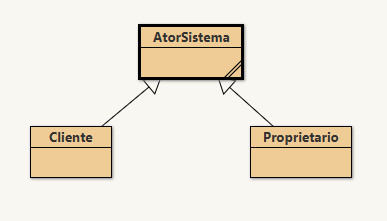
\includegraphics[scale=0.8]{atorsistema.png}
        \label{img:logo}
        \caption{Hierarquia de Utilizadores}
    \end{figure}
    
\subsection{Cliente}
   
\hspace{0.50cm} O que distinguia um Cliente era a sua Localização (Coordenadas X, Y no plano 2D). Por outro lado os Clientes têm uma lista de alugueres que ainda não foram classificados, sendo estes removidos aquando a sua classificação.

\begin{lstlisting}[language=java]

public class Cliente extends AtorSistema {

    private Localizacao coordenadas;
    private List<Aluguer> naoClassificado;
    ...
}
\end{lstlisting}

\subsection{Proprietario}

\hspace{0.50cm} O proprietário possui, no seu estado interno, a sua coleção de veículos. A implementação é simples, um Map cuja \textit{key} é a matrícula do veículo, e o valor é o Objecto Veiculo respetivo (classe que será descrita mais à frente). Também possuem uma lista de alugueres pendentes (ou seja, ainda não aceites).

\begin{lstlisting}[language=java]

public class Proprietario extends AtorSistema{

    private Map<String,Veiculo> mapVeiculos;
    private List<Aluguer> pedidosAluguer;
    ...
}
\end{lstlisting}

\section{Veículo}

\hspace{0.50cm} Os proprietários que têm acesso à aplicação UM carro já! têm à sua disposição variadíssimas funcionalidades, entre elas, poderem adicionar um veículo à sua coleção. Para tal foi necessário criar o objeto Veículo que possui os requisitos básicos de amdmissão nesta aplicação, tais como, uma identificação única, uma localização e propriedades fundamentais, como por exemplo, a velocidade média, preço, etc...

\vspace{0.5cm}

É de realçar que o grupo considerou, numa fase inicial, usar uma variável de instância \textbf{'disponivel'} que indicaria se o veículo estaria disponível no momento de aluguer. Ora visto que os alugueres são instantâneos, tal não foi necessário.

Também é de notar que a classe Veículo é abstrata, o que implicou que todas as suas subclasses implementassem um método em específico que altera a localização do veículo.

\begin{lstlisting}[language=java]

private String marca;
    private String matricula;
    private double velMediaPorKM;
    private double precoPorKm;
    private int classificacao;
    private Localizacao local;
    private String proprietario;
    private int vezesAlugado;
    //private boolean disponivel; --obsoleto
    ...
}

\end{lstlisting}

\subsection{VeiculoComAutonomia}

\hspace{0.50cm} A classe Veículo é, assim, o topo da hierarquia de veículos, visto que contém os requisitos mínimos para um objeto ser admitido como veículo na nossa Aplicação.
Por outro lado, os veículos pré-definidos de UMcarroJá!, são todos veiculos com autonomia. A autonomia funciona, em termos gerais, como o número de kilómetros que o veículo ainda pode percorrer sem a esgotar.

\vspace{0.5cm}

Em termos deste tipo de veículos, temos 3 tipos disponiveis, Veiculos Hibridos, Eletricos e a Gasolina. Apesar desta diferenciação meramente textual, estes possuem um estado interno identico, pois a estrutura desta aplicação (descrita no enunciado) assim o exige.

    \begin{figure}[H]
    \vspace{0.5cm}
        \centering
        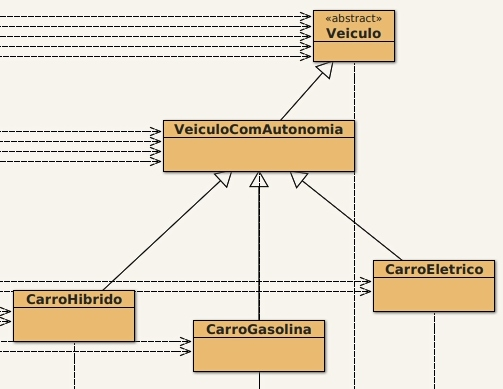
\includegraphics[scale=2]{veiculoGraph.jpg}
        \label{img:logo}
        \caption{Hierarquia de Veículos}
    \end{figure}
   

\section{Localização}

\hspace{0.50cm} Esta foi a classe adotada para representar as coordenadas GPS de um veículo ou de um cliente. Nesta classe apenas são definidos dois double um que representa as coordenadas em x e um outro que representa as coordenadas em y.

\begin{lstlisting}[language=java]

public class Localizacao implements Serializable {

    private double x;
    private double y;
    ...
}    
\end{lstlisting}

\section{Aluguer}

\hspace{0.50cm} A ideia da aplicação reside no facto de um cliente poder alugar um carro de um proprietário, com base em critérios por ele escolhidos. Com vista a este fim implementamos portanto a classe aluguer que guarda a informação de todos os intervenientes do aluguer. Esta classe tem váriáveis de instância como Strings que contêm a identificação dos intervenientes, ou seja, o cliente, o proprietário e o veículo, um double para a distância que foi percorrida, um double para o preço, um LocalDate para a data em que ocorreu o aluguer e uma Localizacao que contém o destino da viagem.

\vspace{0.5cm}

Esta classe vai ser importante para poder ser representada numa lista para classes como por exemplo o cliente
e com o qual poderemos saber todo o seu histórico de movimentos, carro alugado, destino, etc...

\begin{lstlisting}[language=java]

public class Aluguer implements Serializable {

    private String veiculo;
    private String cliente;
    private String proprietario;
    private double distancia;
    private double preco;
    private LocalDate data;
    private Localizacao destinoViagem;
    ...
}
\end{lstlisting}

\section{Comparators}

\hspace{0.50cm} Como as nossas classes podiam ser ordenadas de inúmeras formas (a classe Veículo é um exemplo disso), foi necessário criar \textit{Comparators} consoante os critérios de ordenação adotados.

\subsection{ComparatorVeiculoPrecoKm}

\hspace{0.50cm} Este \textit{Comparator} surge pois pretendia-se uma ordenação de Veículos por preço por kilómetro. Este compara os Veículos ordenando-os por ordem decrescente de preço.

\subsection{ComparatorClientekmPercorridos}

\hspace{0.50cm} Já para ser determinado o \textit{Top} 10 de clientes que percorreram mais km, achamos por bem criar outro comparator. Neste o método compare recebe dois clientes e vai compará-los olhando para o número total de km percorridos por cada um. No caso da função \textit{top10clientes()} é criado um conjunto de clientes e estes estão ordenados por ordem decrescente do número total de km percorridos. 

\section{EstadoSistema}

\hspace{0.50cm} Esta classe serve de base de dados da nossa aplicação. Possui associações em Maps que armazenam os clientes, os proprietários e os veículos registados. Tal é necessário pois é preciso manipular esses dados e apresentar resultados a partir deles.

\vspace{0.5cm}

Por exemplo para uma função que consulte a faturação de um dado veiculo, seria necessário saber qual a identificação desses veiculo (matrícula) e encontrar o seu valor na associação (Map), para depois ser possível percorrer o seu histórico de alugueres e determinar assim a sua faturação. 

\begin{lstlisting}[language=java]

public class EstadoSistema implements Serializable {

    private Map<String, Cliente> clientes_Sistema;
    private Map<String, Proprietario> proprietarios_Sistema;
    private Map<String, Veiculo> veiculos_Sistema;
    ...
}
\end{lstlisting}
 
Na imagem apresentada a seguir pode-se verificar que, aliado à classe \textbf{EstadoSistema} temos a classe \textbf{GestorFicheiroDados} que contém o código necessário para a leitura e inicialização do estado da aplicação. O código foi separado pois possui uma \textit{sintax} diferente do código do modelo da aplicação.
 
   \begin{figure}[H]
    \vspace{0.5cm}
        \centering
        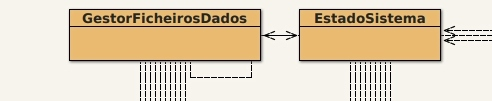
\includegraphics[scale=3]{estado.jpg}
        \label{img:logo}
        \caption{Estado do sistema e Gestor de dados}
    \end{figure}

\section{Exceptions}

\hspace{0.5cm}Como existe muito a procura de utilizadores, de veículos de proprietários, de alugueres, da existência ou não de resposta aos pedidos de \textit{users} é necessário ter o programa preparado para eventuais \textit{null}.
Para isso foram criadas algumas exceções para lidar com eventuais erros, como por exemplo \textit{ClientNotFoundException},  \textit{AtorAlreadyExistsException}, etc...

\chapter{Descrição da aplicação desenvolvida}

\section{Breve introdução}

\hspace{0.50cm} A nossa aplicação ‘UM Carro Já!’ permite que hajam vários utilizadores, sejam eles Proprietários de Veículos disponíveis para alugar, bem como Clientes. Estes utilizadores interagem entre si, no sentido em que o cliente pretende alugar um carro para a sua viagem e o Proprietário do veículo gere o abastecimento do veiculo e aceita ou não os alugueres pedidos.

\section{Menu de log-in, registar e salvar aplicação}

\hspace{0.5cm}Assim, após o início da aplicação, possibilitamos ao utilizador entrar na sua conta, seja ele um Proprietário ou um Cliente. Para além de fazer login, o utilizador pode também fazer “save” de todas as suas interações com o programa, isto para caso o utilizador saia da aplicação, ser possível recuperar todas os alugueres feitos, todos carros inseridos, novas contas, etc...

   \begin{figure}[H]
    \vspace{0.5cm}
        \centering
        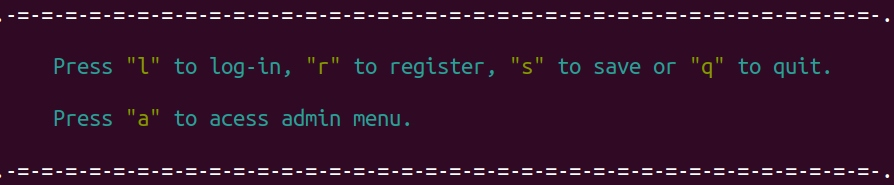
\includegraphics[scale=1.5]{base_images/login.jpg}
        \label{img:logo}
        \caption{Menu incial do utilizador}
    \end{figure}
Após qualquer login ou registo, os clientes/proprietários têm acesso ao seu perfil na aplicação, bem como ao menu de funcionalidades da mesma.
   \begin{figure}[H]
        \centering
        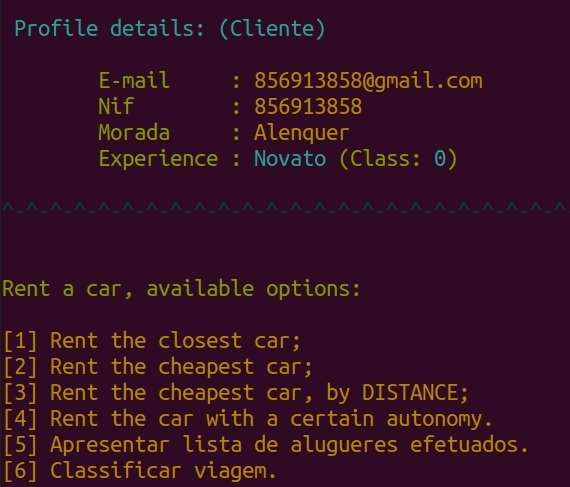
\includegraphics[scale=1.2]{base_images/cliente.jpg}
        \label{img:logo}
        \caption{Exemplo de perfil de um Cliente}
    \end{figure}

\section{Funcionalidades para Clientes e Proprietários}
A nível do Cliente, este pode pedir um aluguer de um carro consoante as suas necessidades e preferências, por exemplo, o carro mais próximo, o carro mais barato, o carro mais barato consoante a distância que está disposto a andar a pé, etc...
Para além de alugar um carro, o cliente pode ver a sua lista de alugueres efetuados, num determinado período, bem como classificar a viagens efetuadas.

\vspace{0.5cm}

A nível de Proprietário, pode aceder à sua lista de veículos para alugar, a lista de alugueres feitos, abastecer veículos, inserir novas viaturas ao sistema do ‘UM Carro Já!’, aceitar/rejeitar pedidos de alugueres por parte de Clientes e consultar a faturação de uma viatura num período de tempo (entre duas datas).

   \begin{figure}[H]
        \centering
        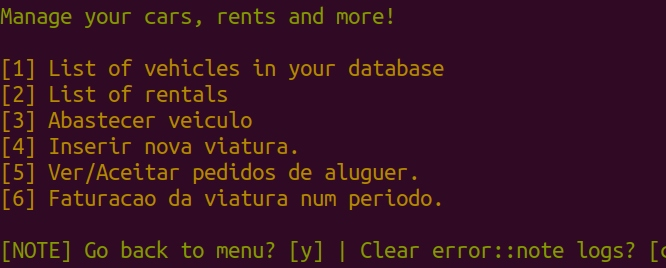
\includegraphics[scale=2]{base_images/propperfil.jpg}
        \label{img:logo}
        \caption{Funcionalidades de um proprietário}
    \end{figure}
    
\vspace{0.5cm}
\section{Exemplos de funcionalidades}

\hspace{0.5cm} 1) Apresentação de um veículo disponivel, bem como informações relevantes como a distância ao cliente, preço do veículo, etc.. :
   \begin{figure}[H]
        \centering
        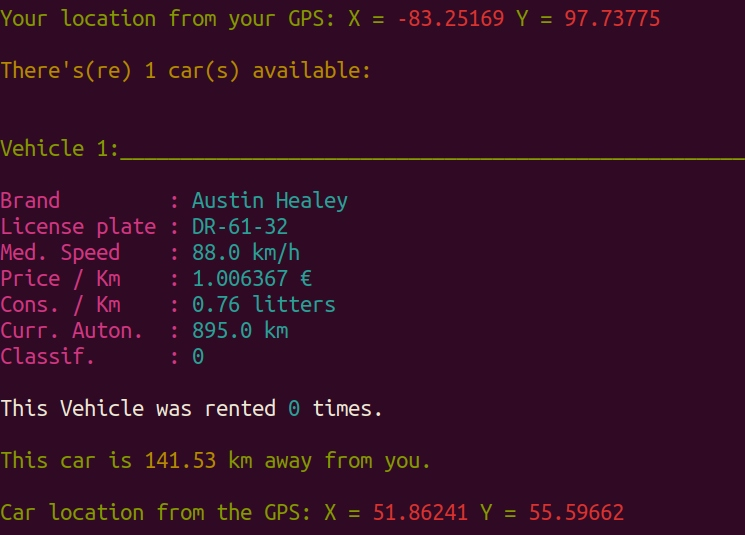
\includegraphics[scale=1.3]{base_images/disponivel.jpg}
        \label{img:logo}
        \caption{Informações de veículo disponível}
    \end{figure}
   \vspace{3cm} 
2) Inserir novas viaturas, consoante o tipo de veículo, por parte de um Proprietário:

   \begin{figure}[H]
        \centering
        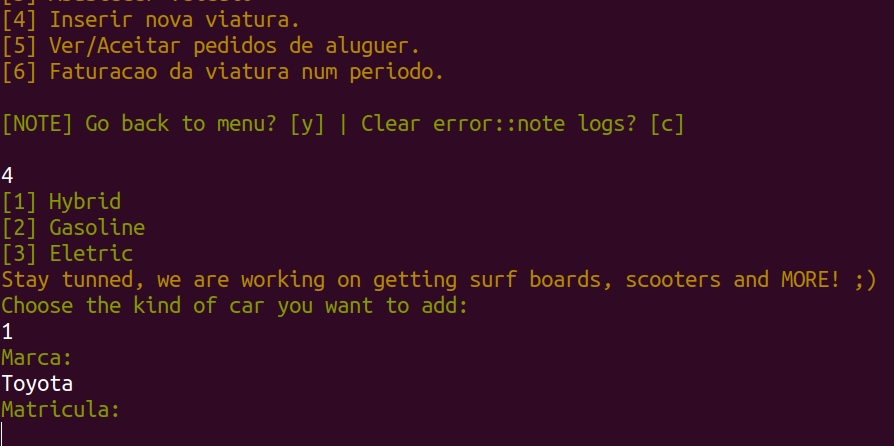
\includegraphics[scale=1.3]{base_images/insert.jpg}
        \label{img:logo}
        \caption{Inserir novo veículo}
    \end{figure}

\section{Registos, Logs e Saves}

\hspace{0.5cm} Voltando ao menu principal é de realçar que a aplicação é, no seu estado inicial, carregada a partir do ficheiro de Logs disponibilizado, no entanto, caso a mesma já possua um registo de \textit{save}, o estado é carregado a partir daí a não ser que esse save seja removido. Seguem-se as diferenças entre uma inicialização com e sem \textit{saves}.

   \begin{figure}[H]
        \centering
        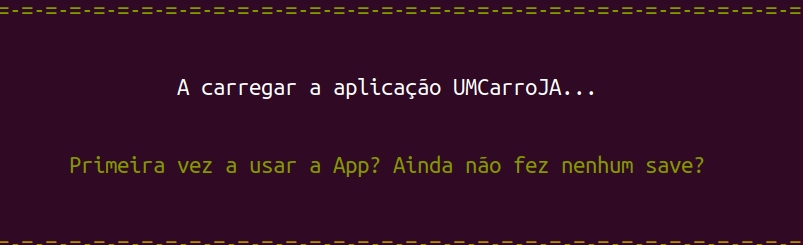
\includegraphics[scale=1.3]{base_images/nosave.jpg}
        \label{img:logo}
        \caption{Inicialização da aplicação \textbf{sem saves}}
    \end{figure}
    
   \begin{figure}[H]
        \centering
        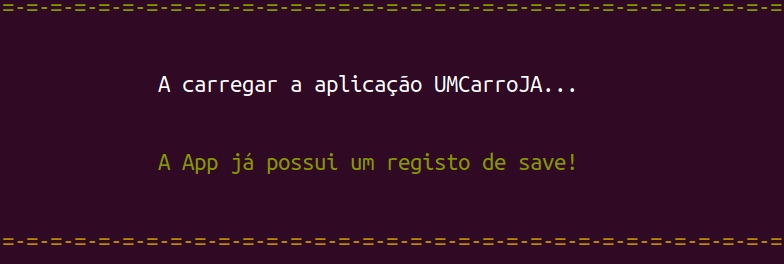
\includegraphics[scale=1.3]{base_images/comsave.jpg}
        \label{img:logo}
        \caption{Inicialização da aplicação \textbf{com saves}}
\vspace{2cm}
    \end{figure}

\section{Ranking de clientes e estatísticas do Sistema}

\hspace{0.5cm} Existem também formas de verificar o ranking de clientes com mais kilómetros percorridos e o número de intervenientes do sistema, acedendo à parte do administrador no menu inicial.

   \begin{figure}[H]
        \centering
        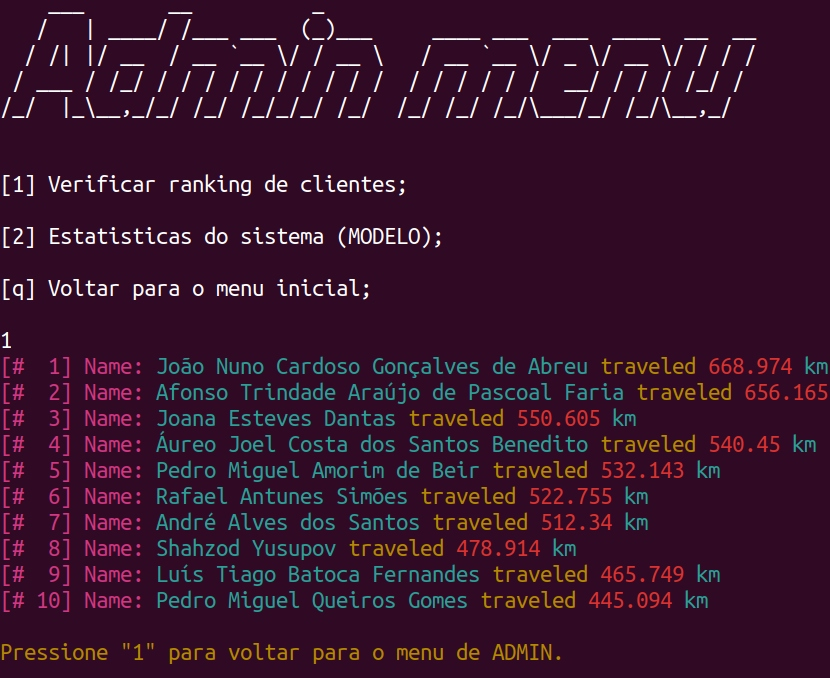
\includegraphics[scale=1.3]{base_images/adminTop.jpg}
        \label{img:logo}
        \caption{Menu de administrador - Ranking de clientes}
    \end{figure}

\section{Visão geral}
%%FIMMMMMM
\vspace{0.5cm}
\par \hspace{0.5cm} Em termos estéticos e de interatividade, a aplicação possui uma série de menus que permitem uma fácil interação com os mesmos, ou seja, ajudam o utilizador a escolher que opções desejam e estão preparados para lidar com eventuais \textit{InputMismatch} por parte dos \textit{users}. É de realçar que não existem programas \textbf{à prova de bala} não sendo este uma exceção!

\chapter{Novos tipos de viaturas na aplicação}

\hspace{0.50cm} Antes de mais, é importante realçar que o grupo tomou um especial cuidado no que toca à hierarquia de classes desta aplicação. Para tal foi necessário decidir, numa fase priliminar, quais seriam os pontos em comum que definiam diferentes veiculos, para isso, fizemos um estudo prévio de quais as variaveis de instância que todos teriam em comum.

\vspace{0.5cm}

A conclusão é simples, para ser veículo tem de ter, no mínimo, uma identificação única (matrícula), uma localização e propriedades que o definem (velocidade, consumo,...). Ora, para adicionar um novo tipo de veiculo, é apenas preciso adicionar uma classe nova, que seja subclasse de Veiculo e essa classe apenas tem de ter o pré-requesito de ter as propriedades básicas de um veiculo.

\vspace{0.5cm}

Nisto, conclui-se, que qualquer tipo de veiculo, em geral, é subclasse de Veiculo e pode facilmente entrar nesta hierarquia.

\chapter{Melhorias na implementação}

\hspace{0.5cm} Após a realização do projeto percebemos que alguns dos problemas que nos foram surgindo resolveram-se com muito mais trabalho do que aquele que seria necessário dada uma boa estruturação do projeto.
\par \vspace{0.5cm}
Ora muitas decisões foram, eventualmente, tomadas apressadamente, e levaram a trazer complexidade desnecessária a problemas simples. Detetado o problema, o grupo considera que este projeto devia ser melhorado em muitos aspetos.

\par \vspace{0.5cm}
Por outro lado, podem não ter sido tomados os melhores métodos de leitura/verificação de \textit{input} do utilizador. Isto pode ter acontecido, talvez por decisões precipitadas ou por inexperiência. No entanto, o facto de termos implementado uma interface baseada no terminal, não nos dá tanta liberdade de recolha de \textit{inputs}, visto que tudo é feito de forma \textbf{sequencial}.

\chapter{Conclusão e prepetivas do trabalho futuro}

\hspace{0.5cm} Em suma, este projeto demonstrou-se como uma mais valia, não só a nível de Programação por Objetos, onde pusemos em prática conceitos adquiridos nas aulas teóricas, mas também na realização de uma aplicação e na proteção dos dados desta. \par
\vspace{0.5cm}
Este trabalho serviu também para assimilar conceitos que a nível teórico tais como a implementação de Interfaces, hierarquia de classes, manipulação de ficheiros, etc..., que se afirmam como elementos chave na utilização de uma linguagem orientada a objetos.
\vspace{0.5cm} \par
Este conceito de encapsulamento que nos foi apresentado neste semestre foi fundamental no desenvolvimento da aplicação, daí que a linguagem orientada a objetos, neste caso java, facilitou-nos na organização do projeto devido às suas regras de estruturação a nível de classes e tipos de dados.
\vspace{0.5cm}\par
Por outro lado, o desenvolvimento desta aplicação foi fundamental para a nossa aprendizagem e para o nosso futuro como Engenheiros Informáticos a nível de organização de código, cooperação em grupo e estrutura do modelo final da aplicação. 
\vspace{0.5cm}\par
Neste último, realçamos a tentativa (que pensamos ter alcançado) a nível da arquitetura ‘MVC’ que separa a representação da informação da interação do utilizador com ela. 
\vspace{0.5cm}\par
Nesta arquitetura temos o módulo dos dados (EstadoSistema) que gere os dados da aplicação, o módulo da interação com o Utilizador (GUI-UMCarroJA) e, por último, o módulo que controla os inputs, convertendo-os em comandos para os outros módulos. Assim, a arquitetura da nossa aplicação defende a ideia da reutilização de código e separação de conceitos.

\end{document}